\documentclass[a4paper,twoside,11pt]{article}
\usepackage{a4wide,graphicx,fancyhdr,amsmath,amssymb, enumerate, caption, subcaption, wrapfig}

%----------------------- Macros and Definitions --------------------------

\setlength\headheight{20pt}
\addtolength\topmargin{-10pt}
\addtolength\footskip{20pt}

\newcommand{\HRule}{\rule{\linewidth}{0.5mm}} % Defines a new command for the horizontal lines,
\newcommand{\N}{\mathbb{N}}
\newcommand{\ch}{\mathcal{CH}}

\fancypagestyle{plain}
\fancyhf{}
\fancyhead[LO,RE]{\sffamily\bfseries\large Technische Universiteit Eindhoven}
\fancyhead[RO,LE]{\sffamily\bfseries\large 2IV35 Visualization}
\fancyfoot[LO,RE]{\sffamily\bfseries\large Department of Mathematics and Computer Science}
\fancyfoot[RO,LE]{\sffamily\bfseries\thepage}
\renewcommand{\headrulewidth}{0pt}
\renewcommand{\footrulewidth}{0pt}


\pagestyle{fancy}
\fancyhf{}
\fancyhead[RO,LE]{\sffamily\bfseries\large Technische Universiteit Eindhoven}
\fancyhead[LO,RE]{\sffamily\bfseries\large 2IV35 Visualization}
\fancyfoot[LO,RE]{\sffamily\bfseries\large Department of Mathematics and Computer Science}
\fancyfoot[RO,LE]{\sffamily\bfseries\thepage}
\renewcommand{\headrulewidth}{1pt}
\renewcommand{\footrulewidth}{0pt}


\begin{document}
\begin{titlepage}

\center % Center everything on the page

\textsc{\Huge \textbf{Technische Universiteit Eindhoven}}\\[1.5cm] % Name of your university/college
\textsc{\LARGE \textbf{Visualization}}\\[0.5cm] % Major heading such as course name
\textsc{\large 2IV35}\\[0.5cm] % Minor heading such as course title

\HRule \\[0.4cm]
{ \huge \bfseries Volume rendering}\\[0.4cm] % Title of your document
\HRule \\[1.5cm]

\begin{minipage}{0.4\textwidth}
\begin{flushleft} \large
\emph{\textbf{Author:}}\\
Sander Kools \\
0848523 \\
s.w.a.kools@student.tue.nl % Your name
\end{flushleft}
\end{minipage}
~
\begin{minipage}{0.4\textwidth}
\begin{flushright} \large
\emph{\textbf{Author:}}\\
Luuk Hulten\\
0720248 \\
l.a.j.v.hulten@student.tue.nl
\end{flushright}
\end{minipage}\\[4cm]

{\large \today}\\[3cm] % Date, change the \today to a set date if you want to be precise

\vfill % Fill the rest of the page with whitespace

\end{titlepage}

\newpage
\tableofcontents
\newpage

\section*{Introduction}
In this report we will describe some implementation details of the volume rendering application. We will show the advantages and disadvantages of some rendering techniques at the hand of images.
In section 1, we will give some details about rendering in a lower resolution to speed up interacting with the application. \newline
In section 2, we will . \newline
In section 3, we will . \newline
In section 4, we will . \newline
Finally in section 5, we will give a short conclusion about how we choose to visualize the data. \newline

\section{Speeding up interaction}
Since most visualization techniques are quite slow, interacting with the visualization becomes laggy and difficult. To speed up these interaction we render the image while interacting in a lower resolution. We implemented the rendering to render the image in three different resolutions. These resolutions are $\frac{1}{4}$ and $\frac{1}{2}$ of the original resolution. At last we render the image at full resolution.
This enables the user to interact with the image and see some result in low detail. For example when rotating the users sees the image in $\frac{1}{4}$ of the resolution. When he stops rotating the image is rendered at $\frac{1}{2}$ of the resolution this image is well enough for the user to determine if this is the view he liked. After the calculation is completed the image is rendered at full resolution.
Normally calculating in three resolutions introduces extra overhead but since intermediate results are stored little overhead is introduced.
Also the calculation of the pixels is done multi threaded this means that the user can interact with the visualization while pixels are been calculated. While interacting while pixels are calculated the pixel queue is cleared and filled with the pixels of the new visualization.

\begin{figure}[h]
\begin{center}
        \begin{subfigure}[b]{0.23\textwidth}
                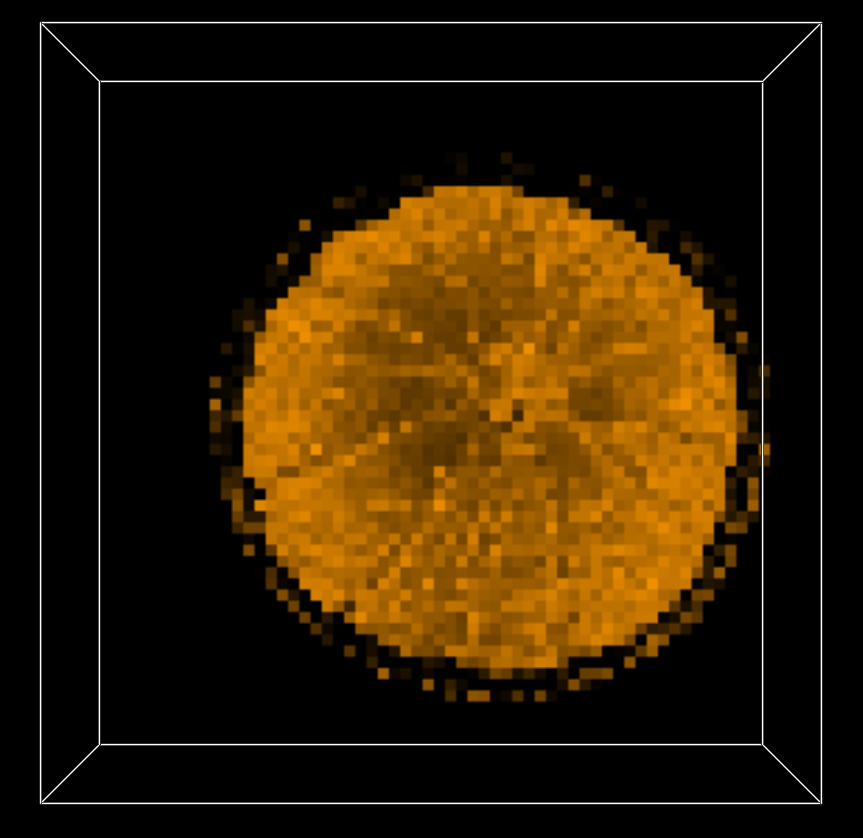
\includegraphics[width=\textwidth]{Images/res4.png}
                \caption{$\frac{1}{4}$ Resolution}
                \label{fig:res4}
        \end{subfigure}
        \begin{subfigure}[b]{0.23\textwidth}
                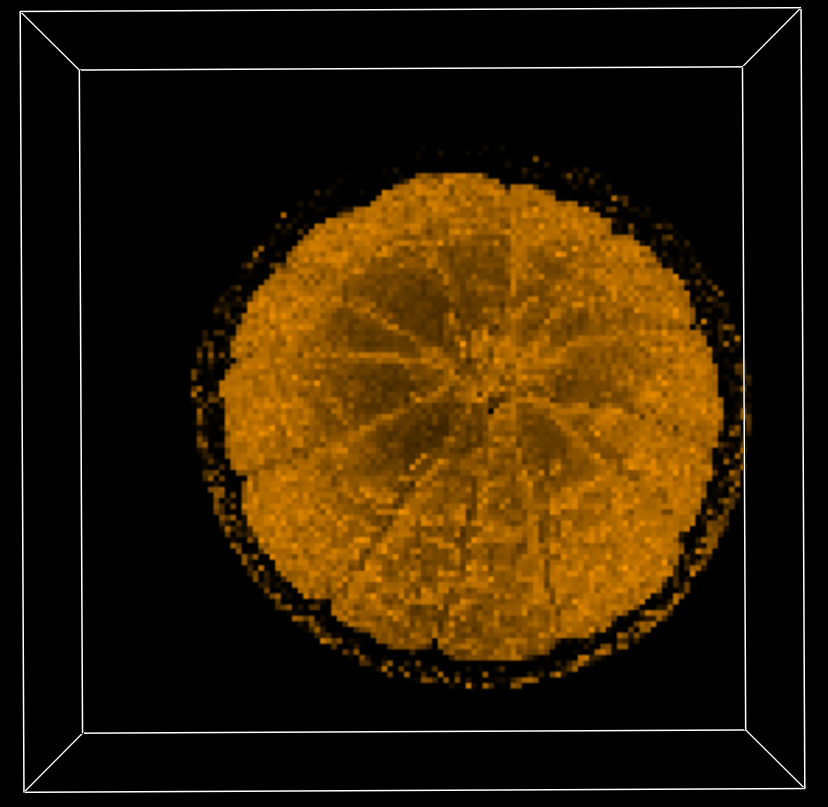
\includegraphics[width=\textwidth]{Images/res2.png}
                \caption{$\frac{1}{2}$ Resolution}
                \label{fig:res2}
        \end{subfigure}
        \begin{subfigure}[b]{0.23\textwidth}
                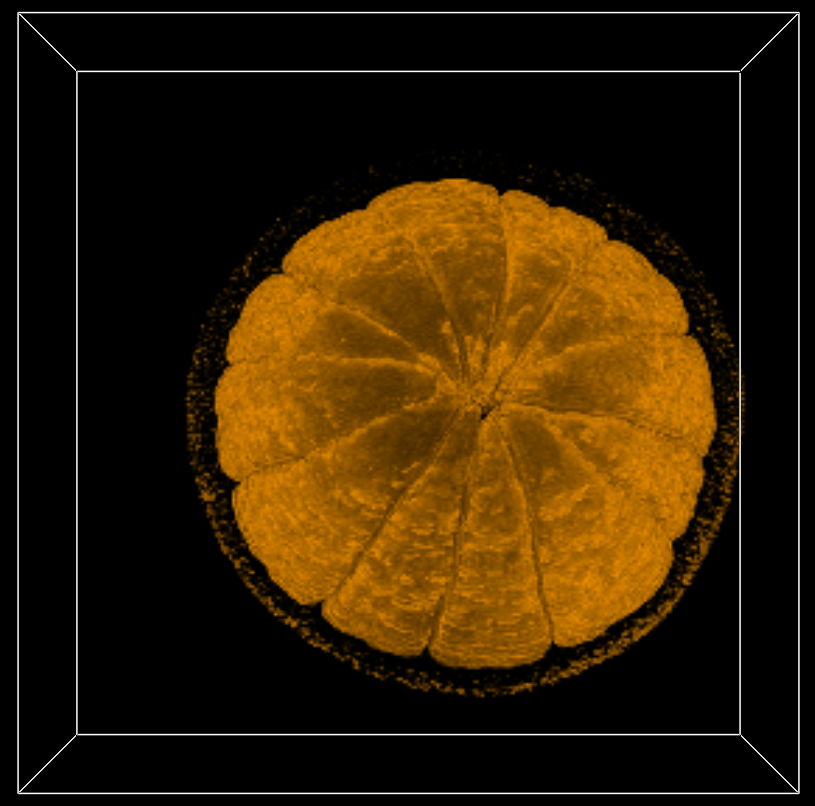
\includegraphics[width=\textwidth]{Images/res1.png}
                \caption{Full resolution}
                \label{fig:res1}
        \end{subfigure}
        \caption{Pie Charts}\label{fig:Resolutions}
\end{center}
\end{figure}


\section{Compositing}
\newpage
\section{MIP}
In scientific visualization, a maximum intensity projection (MIP) is a volume rendering method for 3D data. It consists of projecting the voxel with the highest attenuation value on every view throughout the volume onto a 2D image. \newline
This method tends to display bone and contrast material–filled structures preferentially, and other lower-attenuation structures are not well visualized. The primary clinical application of MIP is to improve the detection of pulmonary nodules and assess their profusion. MIP also helps characterize the distribution of small nodules. In addition, MIP sections of variable thickness are excellent for assessing the size and location of vessels, including the pulmonary arteries and veins. \newline
For the implementation of the MIP we sampled every pixel by casting a ray through the data and set the voxel to the maximum value. First we iterate over every pixel. At every pixel we record the corresponding voxel value and if it's the highest value we've encountered, we save it as being the highest value until we possibly find a higher one later in the iteration. \newline
Below in figure \ref{fig:FishMIP} there is an example of a MIP rendering using the fish dataset and the composition as comparison in figure \ref{fig:FishComp}.
\begin{figure}[h]
    \begin{center}
        \begin{subfigure}[b]{0.47\textwidth}
            \includegraphics[width=\textwidth]{SanderImages/visMIPZ.png}
            \caption{Fish MIP rendering}
            \label{fig:FishMIP}
        \end{subfigure}
        \begin{subfigure}[b]{0.49\textwidth}
            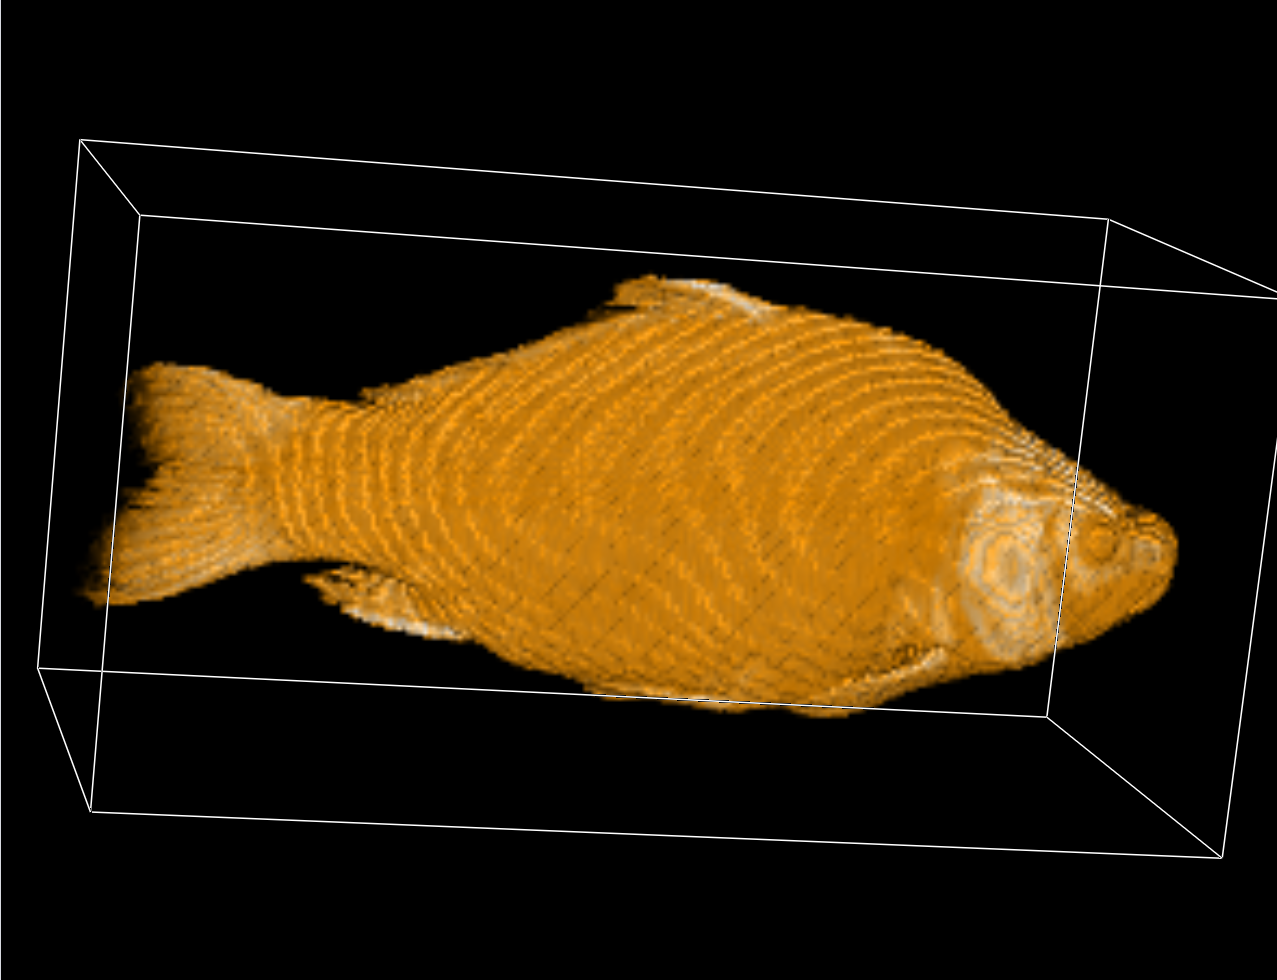
\includegraphics[width=\textwidth]{SanderImages/FishCompZ.png}
            \caption{Fish Composition rendering}
            \label{fig:FishComp}
        \end{subfigure}
        \caption{Fish rendering, MIP and composition}
    \end{center}
\end{figure} \newline
We see that MIP works well when the datasets have objects with high density, such as the Fish or the Skeleton, for instance in figure \ref{fig:PigMIP} you are able to see the contents of the Piggy bank using this rendering form, which wasn't able with the composition rendering.
\begin{figure}[h]
    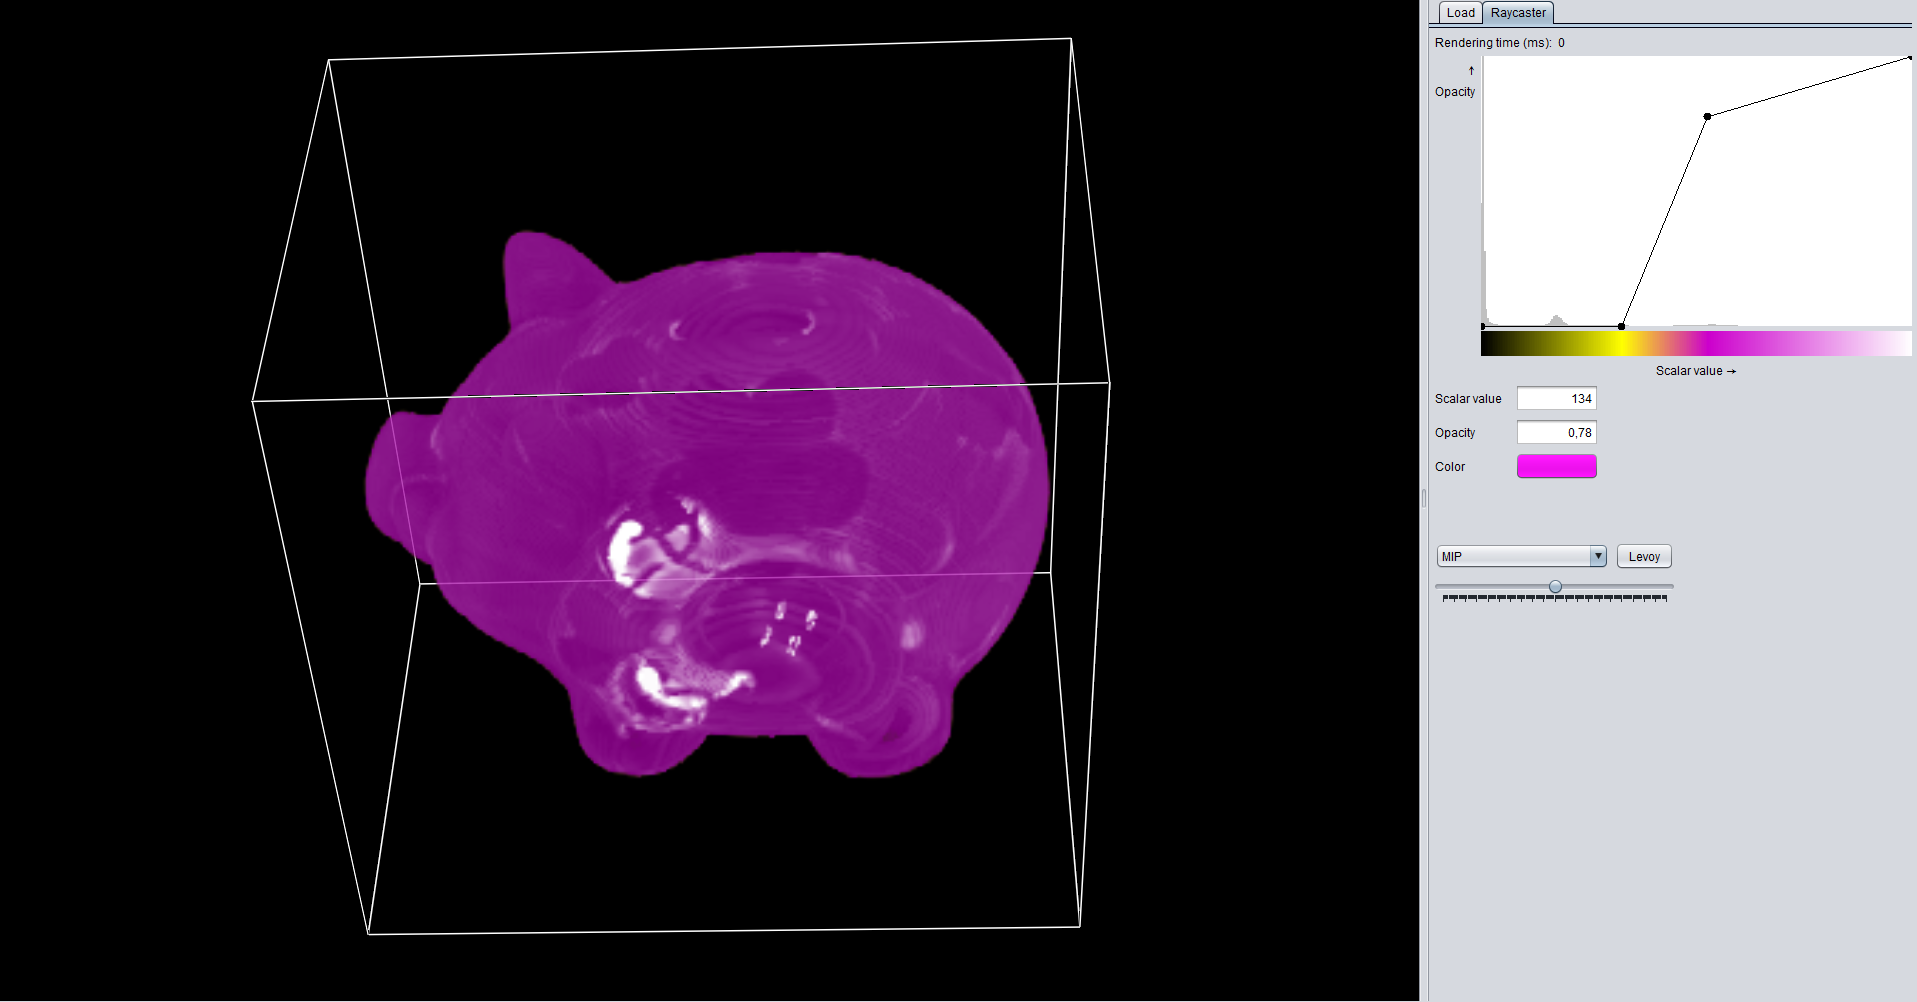
\includegraphics[width=\textwidth]{SanderImages/PigMIP2.png}
    \caption{Pig MIP}
    \label{fig:PigMIP}
\end{figure}

\begin{figure}[h]
    \begin{center}
        \begin{subfigure}[b]{0.32\textwidth}
            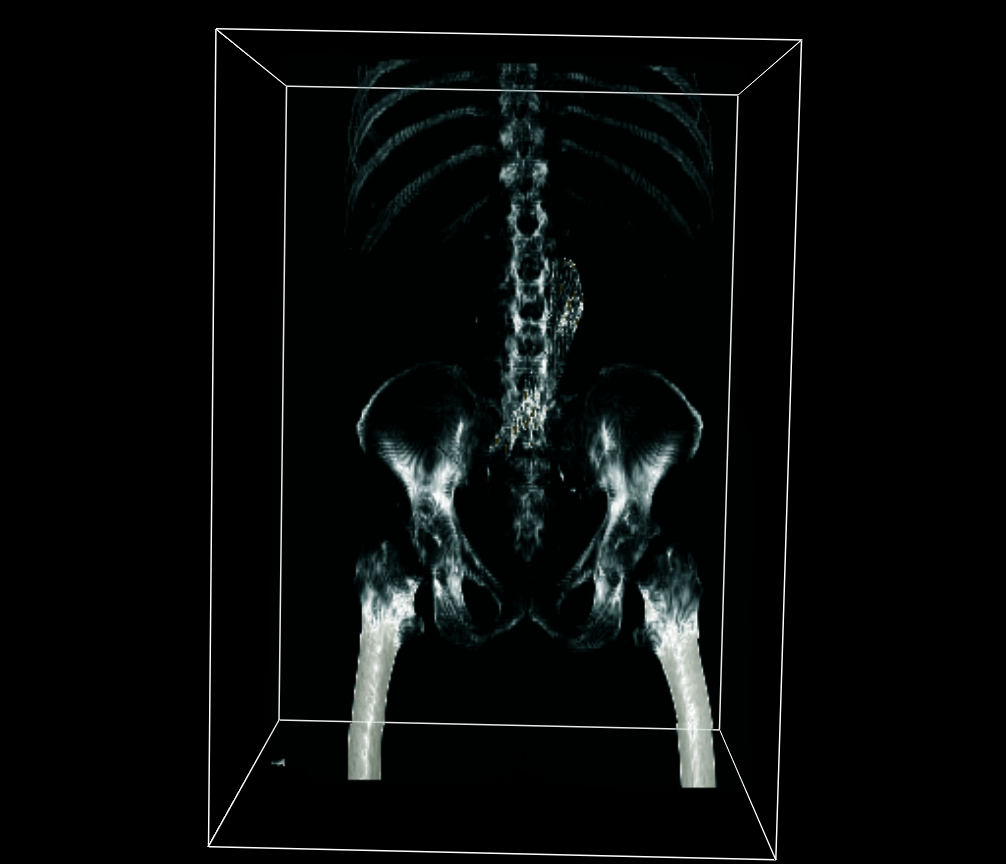
\includegraphics[width=\textwidth]{SanderImages/SkeletonMIPZ.png}
            \caption{Skeleton MIP}
            \label{fig:Skeleton}
        \end{subfigure}
        \begin{subfigure}[b]{0.33\textwidth}
            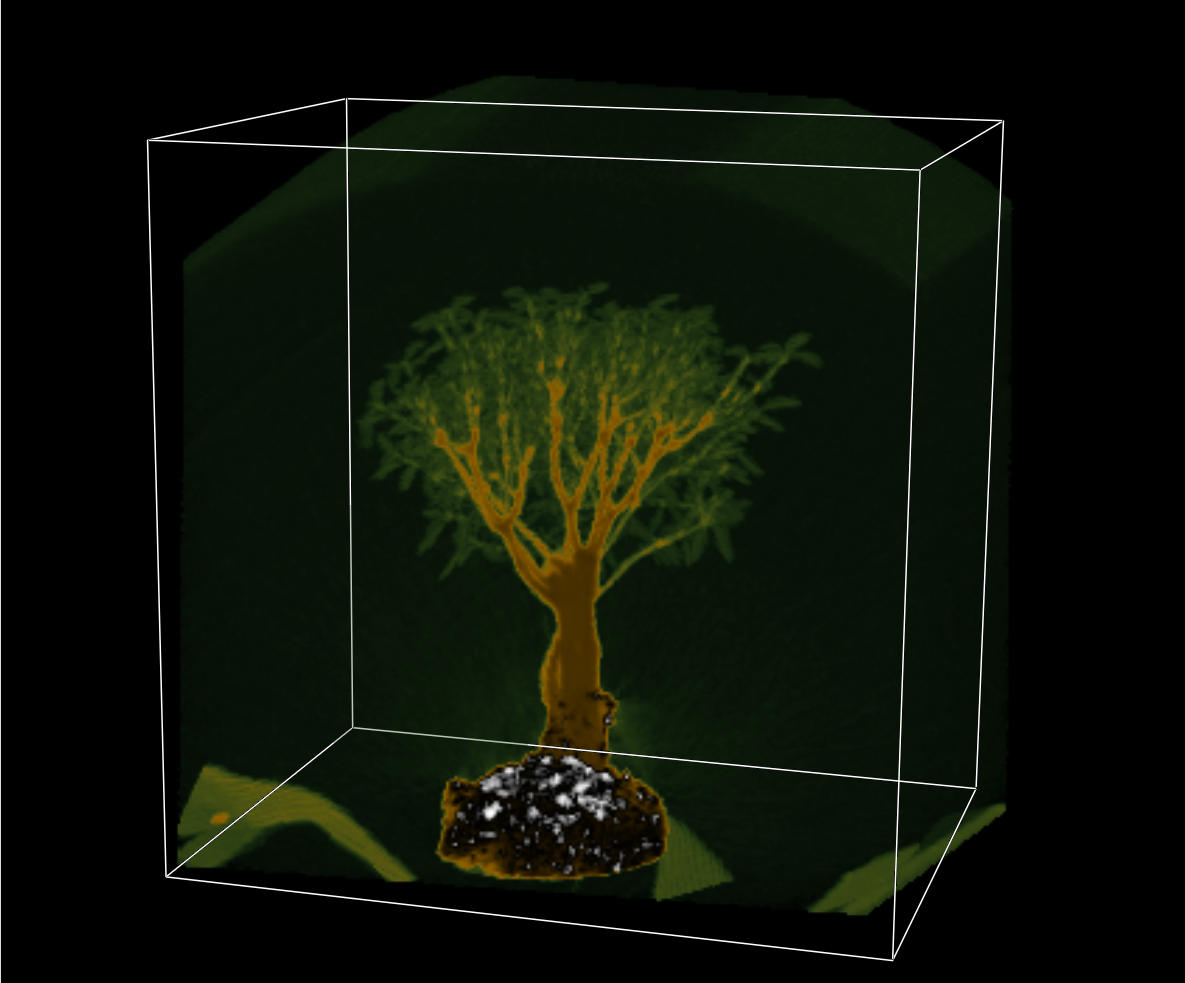
\includegraphics[width=\textwidth]{SanderImages/BonsaiMIPZ.png}
            \caption{Bonsai MIP}
            \label{fig:Bonsai}
        \end{subfigure}
        \begin{subfigure}[b]{0.30\textwidth}
            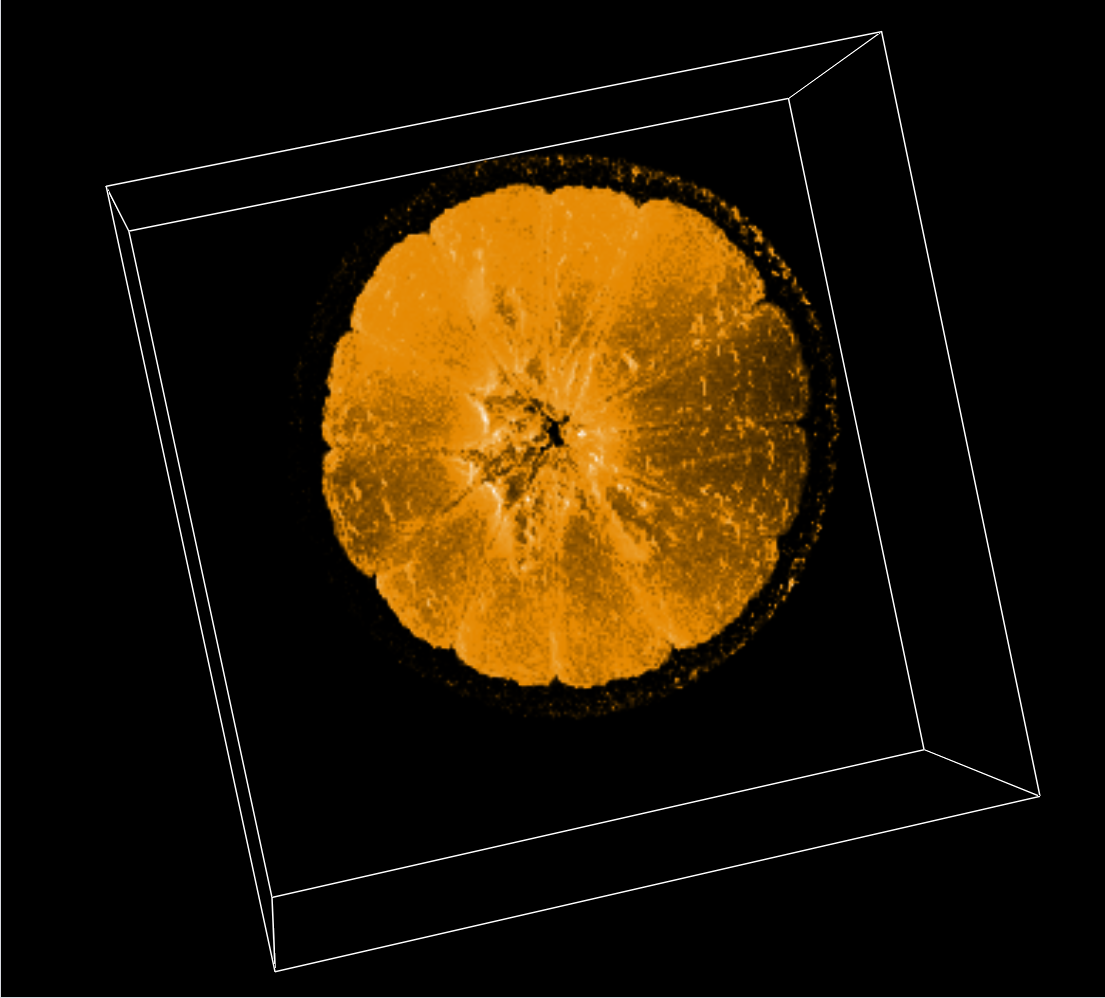
\includegraphics[width=\textwidth]{SanderImages/OrangeMIPZ.png}
            \caption{Orange MIP}
            \label{fig:OrangeMIP}
        \end{subfigure}
        \caption{Multiple MIP renderings}
    \end{center}
\end{figure}
\newpage
\end{document} 